\subsection{Results}

\subsubsection{Deterministic Heuristic Comparison}

We evaluate all heuristics on a cached graph snapshot (41~nodes, 864~edges) from 30 randomly selected start nodes at three cash levels (\$1k, \$10k, \$100k), totalling 90~runs per method. By freezing the graph, we isolate algorithmic differences from API latency. Full results are reported in Table~\ref{tab:heuristic-performance}; we summarise the key findings here.

All A*-based methods achieve identical success rates (56.7\%), confirming that heuristic choice does not affect \emph{whether} a profitable path exists, only \emph{which} path is found and how efficiently. The 3-hop enumeration baseline succeeds for only 30\% of start nodes because it cannot discover 2-hop intra-exchange opportunities or 4+~hop cross-exchange paths.

$h_2$ (slippage) achieves the best search efficiency, reducing node expansions by \textbf{29\%} relative to Dijkstra across all cash levels while matching Dijkstra's profit within 1\% at large order sizes. This demonstrates that order-book depth information provides effective search guidance.

$h_4$ (Weighted~A*) expands 87\% more nodes than Dijkstra due to its chain-congestion and exchange-reliability penalties, but its wall-clock compute time (0.020--0.022\,s) is comparable to Dijkstra's (0.010\,s) because it makes \emph{zero API calls} during search. The additional expansions produce longer paths (5--6~hops) that route through higher-reliability exchanges, trading profit for execution safety.

$h_1$ (liquidity) exhibits cash-size-dependent behaviour: at \$1k it reduces expansions by 11\% (the liquidity ratio is favourable), but at \$100k it expands 99\% more nodes (large orders trigger stronger liquidity penalties, forcing broader exploration).

Start node sensitivity persists across all methods: approximately 43\% of randomly chosen start nodes yield no profitable path regardless of heuristic, reflecting structural properties of the fee landscape rather than algorithmic limitations.

\subsubsection{Comparison Against Baselines}

We compare our heuristic-guided A* methods against five baseline algorithms: Dijkstra's algorithm (A* with $h(n) = 0$), brute-force 3-hop enumeration, Bellman--Ford negative cycle detection, simple 1-hop arbitrage, and simple 2-hop arbitrage with maximum depth constraint (2hop\_max).

\paragraph{3-hop enumeration baseline.}
Since observed optimal paths are consistently 3 hops, we implement a brute-force baseline that exhaustively enumerates all 3-hop paths of the form transfer$\to$trade$\to$transfer and trade$\to$transfer$\to$trade from each start node. On our 12-exchange graph, this baseline evaluates thousands of candidate paths per start node. Its execution time scales as $O(|V| \cdot d^3)$ where $d$ is the maximum out-degree, making it feasible for graphs with $\leq$100 nodes but prohibitive for larger graphs.

The 3-hop baseline finds the \emph{same} optimal paths as our A* heuristics when profitable 3-hop paths exist, confirming that A* does not sacrifice path quality. Because 3-hop enumeration grows as $O(|V| \cdot d^3)$, its node evaluations increase rapidly with graph size, while heuristic-guided A* prunes the majority of candidate paths. Our graph scaling experiments (Section~\ref{sec:graph_scaling}) quantify this divergence: as the number of exchanges increases from 4 to 12, the enumeration baseline evaluates an increasingly larger fraction of the search space compared to heuristic-guided search.

\paragraph{Other baselines.}
Simple 1-hop and 2-hop arbitrage algorithms fail to find profitable paths across all starting nodes and order sizes. This confirms that profitable stablecoin arbitrage requires at least 3 hops.

Bellman--Ford negative cycle detection fails to find profitable cycles in all tested scenarios. This is expected, as our graph construction uses conservative pricing (bid/ask spreads) and includes all execution costs, which eliminates theoretical negative cycles that would exist under idealized pricing assumptions. The failure of Bellman--Ford validates our execution-aware approach.

On the cached graph, Dijkstra computes in ${\sim}$10\,ms per trial, comparable to $h_4$ (20\,ms) and faster than $h_1$/$h_2$ when their API caches miss. In live experiments, Dijkstra's wall-clock time is dominated by graph-building I/O rather than search, narrowing the practical gap. The key distinction is not raw speed but path quality under execution: Dijkstra paths are optimal in static cost, while $h_2$ and $h_4$ paths account for dynamic risks (slippage, chain congestion) that may affect execution outcomes.

\subsubsection{Monte Carlo Backtesting}
\label{sec:mc_experiments}

To assess robustness beyond single-snapshot deterministic experiments, we conduct Monte Carlo backtesting with 500 trials per heuristic across five order sizes (\$100, \$1,000, \$10,000, \$50,000, \$100,000). Each trial randomly selects a start node and order size, building a fresh graph snapshot for each run. This captures temporal variation in market conditions and provides distributional statistics on heuristic performance.

The Monte Carlo framework reports: success rate (fraction of trials finding a profitable path), conditional average profit (mean profit among successful trials), average runtime per trial (with 5-decimal precision), and path-length distribution. The 3-hop enumeration baseline is included in the Monte Carlo evaluation, enabling direct comparison of exhaustive enumeration against A*-guided search across hundreds of independent market snapshots.

\subsubsection{Graph Scaling}
\label{sec:graph_scaling}

To evaluate how search performance scales with graph size, we construct progressively larger graphs by increasing the number of exchanges from 4 to 12 (in increments of 2), yielding graphs ranging from 19~nodes / 161~edges to 41~nodes / 864~edges. For each graph size we run 10~trials per heuristic from randomly selected start nodes.

Table~\ref{tab:graph_scaling} summarises node expansions across graph sizes. Because our heuristics are \emph{guidance penalties} rather than admissible lower bounds (see Section~3), they steer search toward execution-safe paths at the cost of additional node expansions relative to Dijkstra. Dijkstra's expansion count remains relatively flat (341--404) across graph sizes because it terminates as soon as any profitable path is found without evaluating risk. $h_1$ and $h_4$ expand 19--130\% more nodes because the added penalty costs force the search to explore risk-adjusted alternatives before converging.

\begin{table}[t]
\centering
\small
\caption{Mean node expansions by graph size and heuristic (10 trials each).}
\label{tab:graph_scaling}
\begin{tabular}{rrrcccc}
\toprule
\textbf{Exch.} & \textbf{$|V|$} & \textbf{$|E|$} & \textbf{Dijkstra} & $\mathbf{h_1}$ & $\mathbf{h_4}$ & \textbf{3-hop} \\
\midrule
 4 &  19 &  161 & 341 & 407 & 600 & 365 \\
 6 &  28 &  368 & 378 & 758 & 1100 & 662 \\
 8 &  35 &  619 & 387 & 479 & 618 & 378 \\
10 &  39 &  760 & 404 & 577 & 706 & 490 \\
12 &  41 &  864 & 395 & 768 & 910 &  67 \\
\bottomrule
\end{tabular}
\end{table}

The 3-hop enumeration baseline exhibits high variance: at 12~exchanges it evaluates only 67~nodes (the structural pruning of invalid 3-hop patterns becomes very effective in dense graphs), while at 6~exchanges it evaluates 662. This brittleness contrasts with the monotonic scaling of A*-based methods.

Wall-clock time further differentiates the methods. $h_4$ (Weighted~A* with pre-computed chain and exchange risk scores) averages 0.020--0.027\,s per trial regardless of graph size, making it the fastest heuristic-guided method. $h_1$ averages 0.016--0.673\,s because some trials incur live API calls for 24h-volume data. Dijkstra averages ${\sim}2.1$\,s per trial, dominated by data-acquisition overhead rather than search computation. These results support the recommendation (Section~\ref{sec:mc_experiments}) to benchmark on cached snapshots when isolating algorithmic cost.

Figures~\ref{fig:graph_scaling_time} and \ref{fig:graph_scaling_exp} visualise wall-clock time and node expansions as a function of exchange count.

\begin{figure}[t]
    \centering
    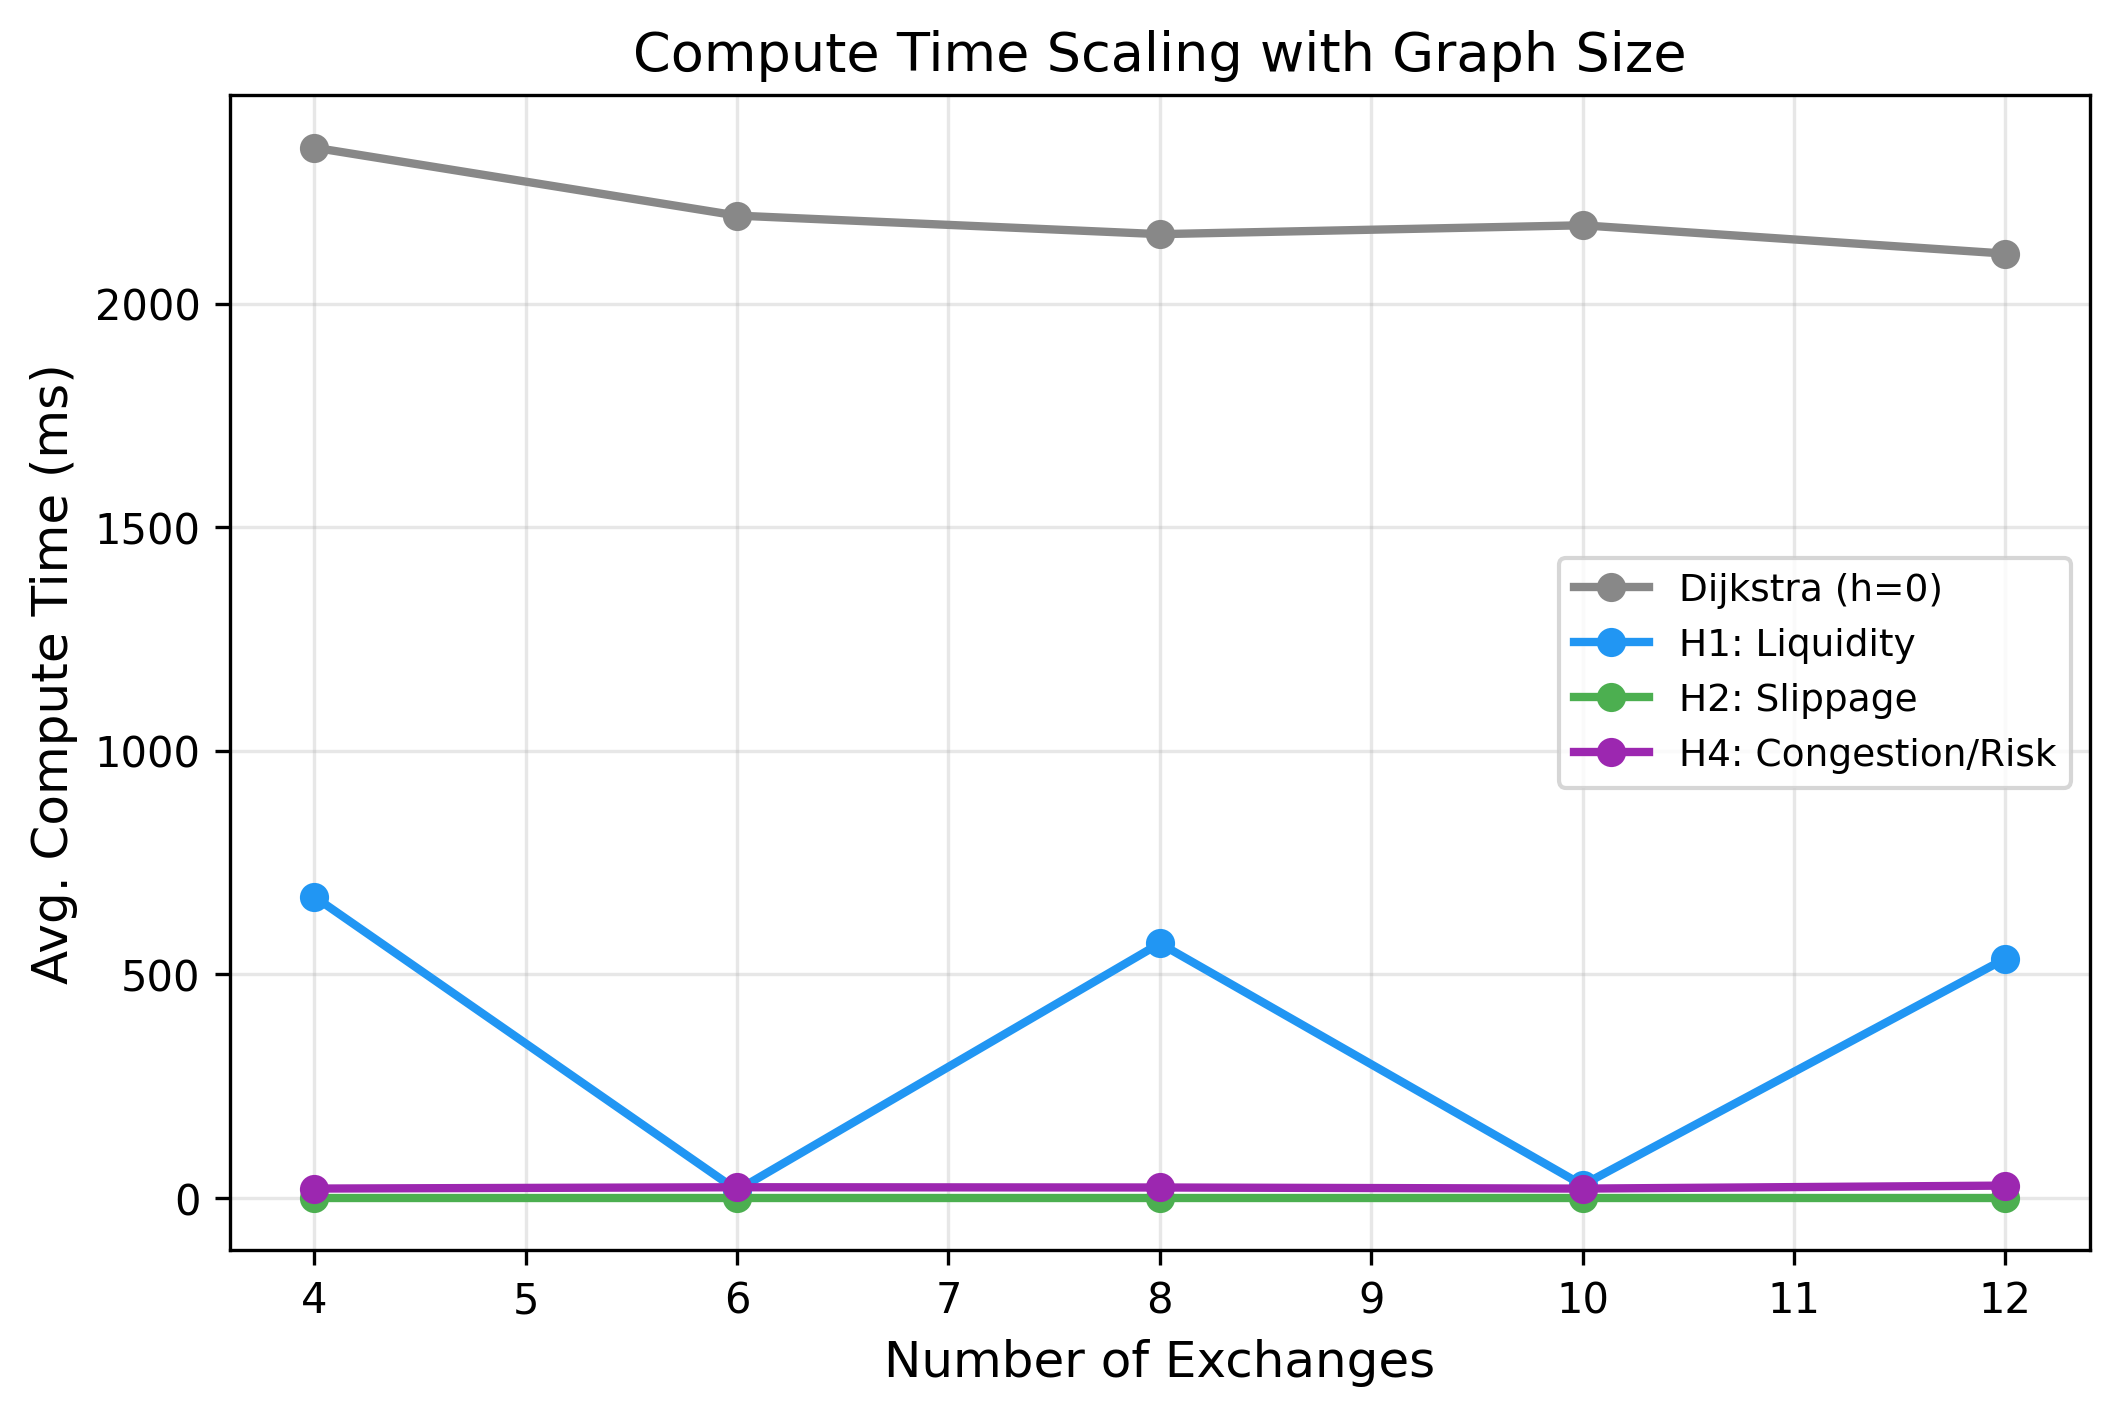
\includegraphics[width=\linewidth]{figures/fig07_graph_scaling_time.png}
    \caption{Mean wall-clock search time vs.\ number of exchanges. $h_4$ maintains sub-30\,ms latency across all graph sizes; Dijkstra's time is dominated by data-fetch overhead.}
    \label{fig:graph_scaling_time}
\end{figure}

\begin{figure}[t]
    \centering
    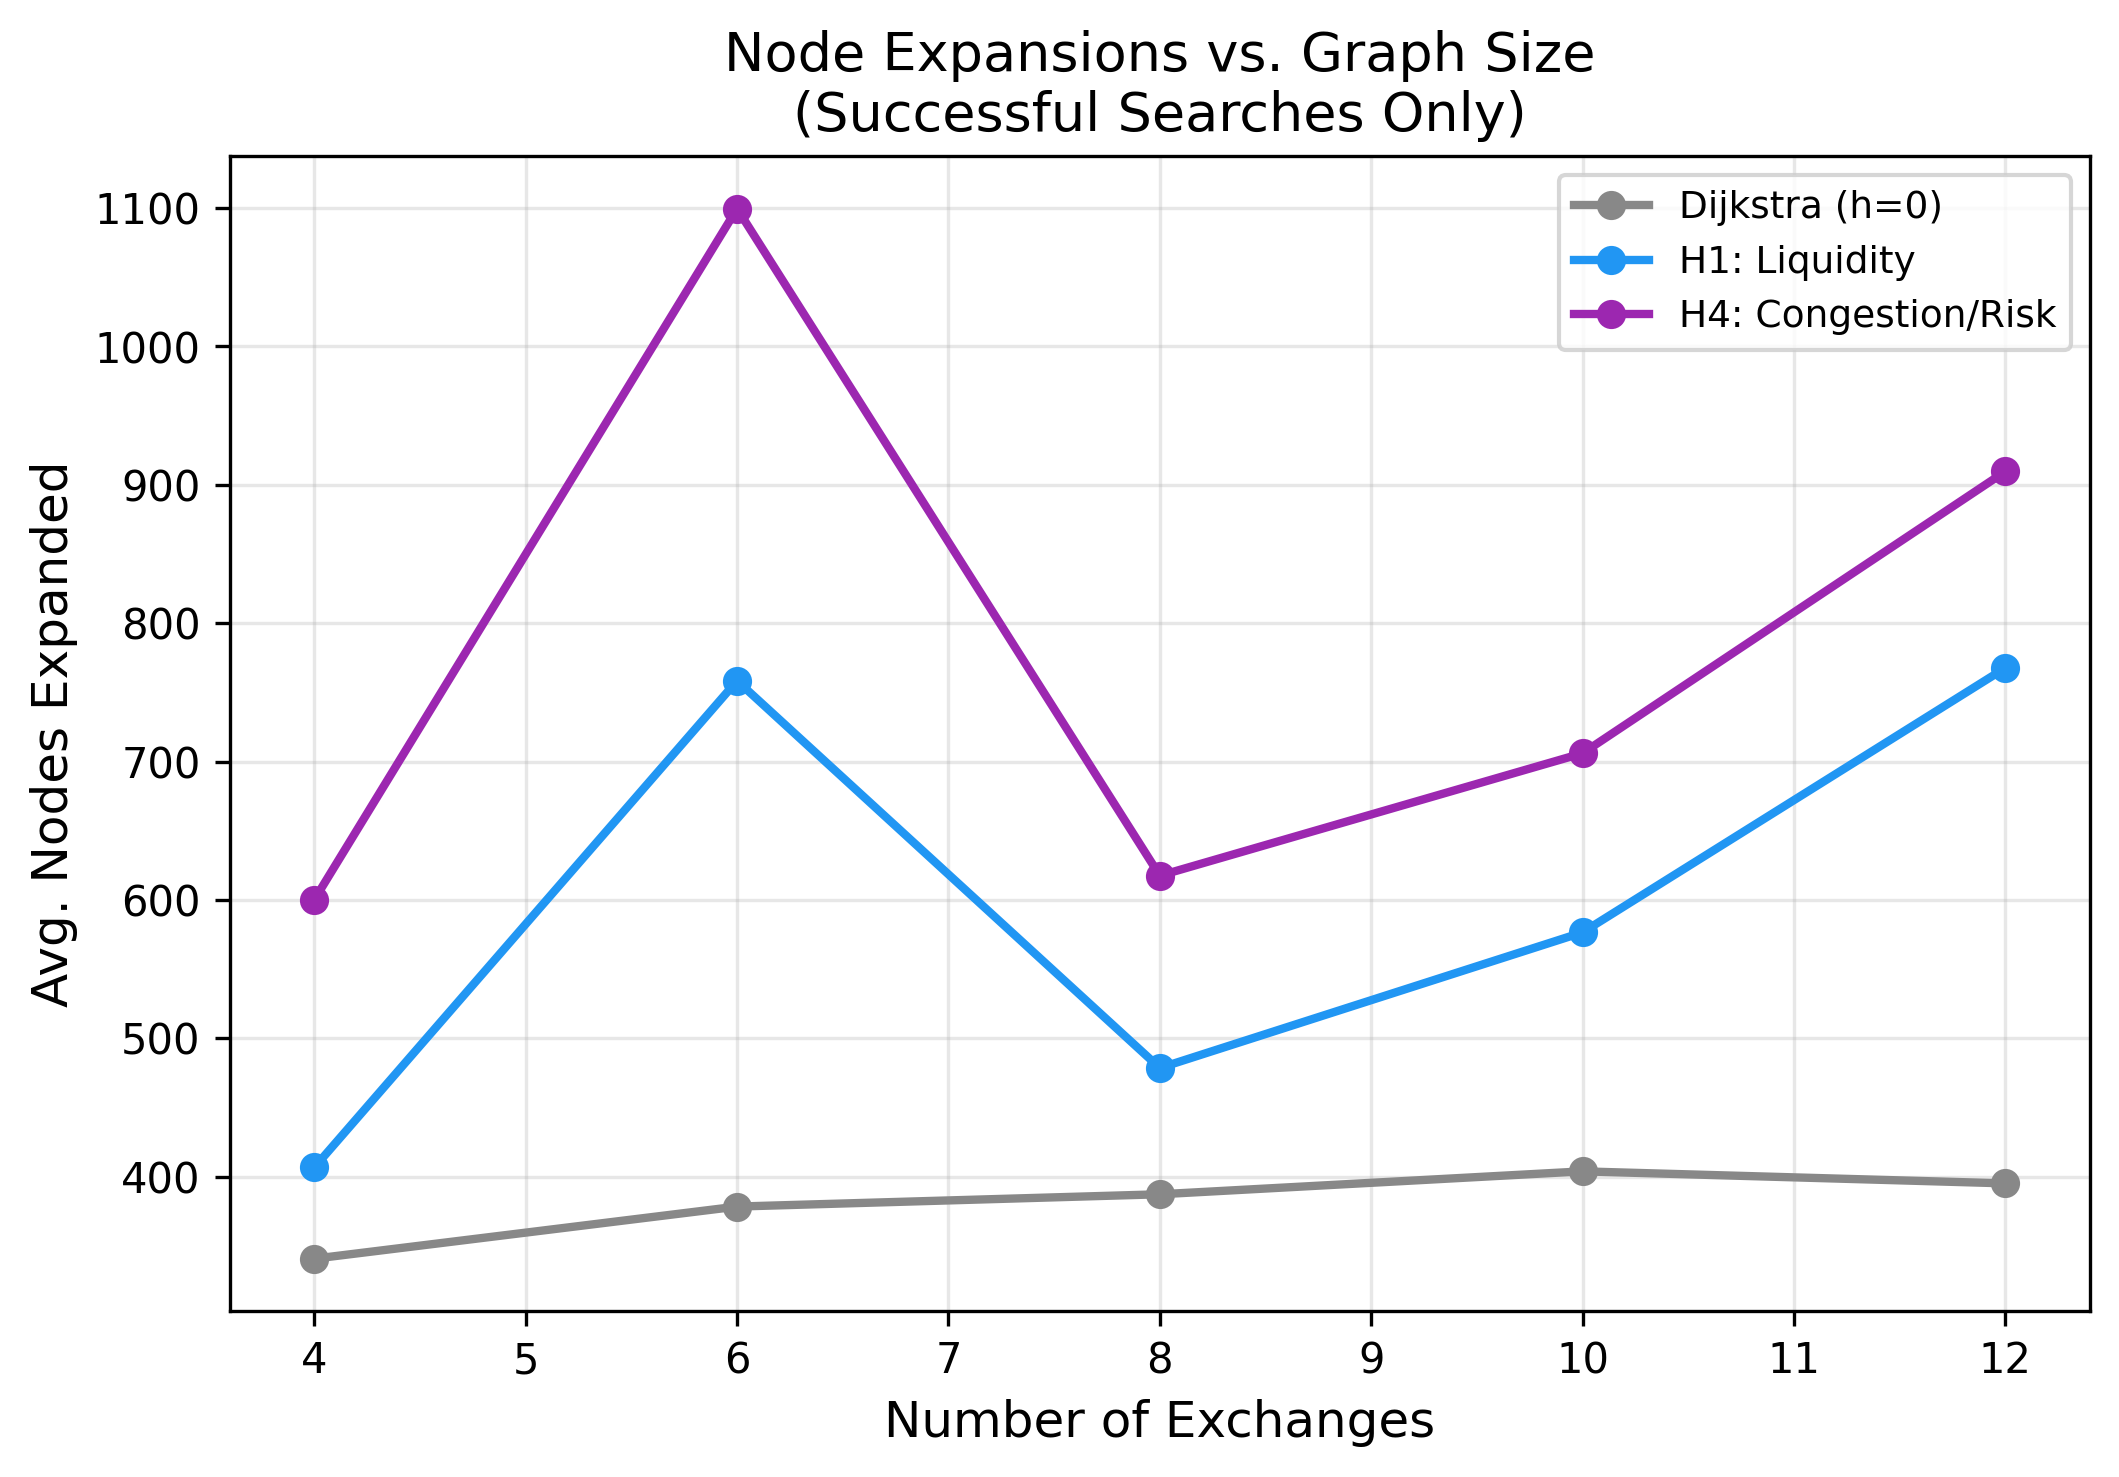
\includegraphics[width=\linewidth]{figures/fig08_graph_scaling_expansions.png}
    \caption{Mean node expansions vs.\ number of exchanges. Heuristic-guided methods expand more nodes than Dijkstra as a consequence of penalty-driven risk exploration.}
    \label{fig:graph_scaling_exp}
\end{figure}

\subsubsection{Quote Staleness and Path Survival}
\label{sec:quote_staleness}

Because the reported margins (${\sim}0.1\%$) are thin, we assess whether identified paths remain profitable under realistic execution latencies. For each of three independent market snapshots, we discover the top profitable paths using $h_1$ and the 3-hop baseline, then re-evaluate each path against \emph{fresh} market data after delays of 5, 10, 30, 60, 120, and 300~seconds.

Across 270 path$\times$delay measurements, \textbf{99.6\%} of paths remain profitable: every path survives delays up to 120\,s, and only at 300\,s does a single path lose profitability (98\% survival). Surprisingly, the mean profit \emph{increases} on re-evaluation at all delay windows (mean ``decay'' is negative: $-55\%$ to $-73\%$), indicating that market microstructure fluctuations frequently improve previously-identified opportunities within the 5-minute window. Table~\ref{tab:staleness} reports per-delay statistics.

\begin{table}[t]
\centering
\small
\caption{Quote staleness: path survival and profit change after re-evaluation at various delays. Negative decay indicates profits increased.}
\label{tab:staleness}
\begin{tabular}{rcrc}
\toprule
\textbf{Delay (s)} & \textbf{Paths} & \textbf{Profitable} & \textbf{Mean Decay (\%)} \\
\midrule
   5 & 45 & 100\% & $-64.6$ \\
  10 & 45 & 100\% & $-67.0$ \\
  30 & 45 & 100\% & $-71.6$ \\
  60 & 45 & 100\% & $-72.7$ \\
 120 & 45 & 100\% & $-72.4$ \\
 300 & 45 &  98\% & $-55.0$ \\
\bottomrule
\end{tabular}
\end{table}

\paragraph{Interpretation and limitations.}
These results demonstrate that stablecoin arbitrage paths exhibit strong \emph{structural} persistence: the fee landscape (fixed withdrawal costs, gas fees, and exchange taker rates) changes slowly, and stablecoin price deviations from the \$1 peg are typically small relative to the fee-determined profit floor.

However, we note an important caveat: re-evaluated profits showed \emph{no variation across delay windows} for the same path within a single round (the re-fetched price for \texttt{okx:USDC} at 5\,s and 300\,s delay was identical to four decimal places). This likely reflects CCXT's internal rate limiting or exchange-side caching of ticker data. Consequently, the survival rates reported above should be interpreted as measuring \textbf{structural path robustness} (whether the fee/rate structure still supports the path) rather than \textbf{price-change robustness} (whether moment-to-moment price fluctuations invalidate the path). A more rigorous replay study using exchange-provided historical tick data would be needed to fully assess price-level staleness risk. Figure~\ref{fig:staleness} visualises path survival rates across delay windows.

\begin{figure}[t]
    \centering
    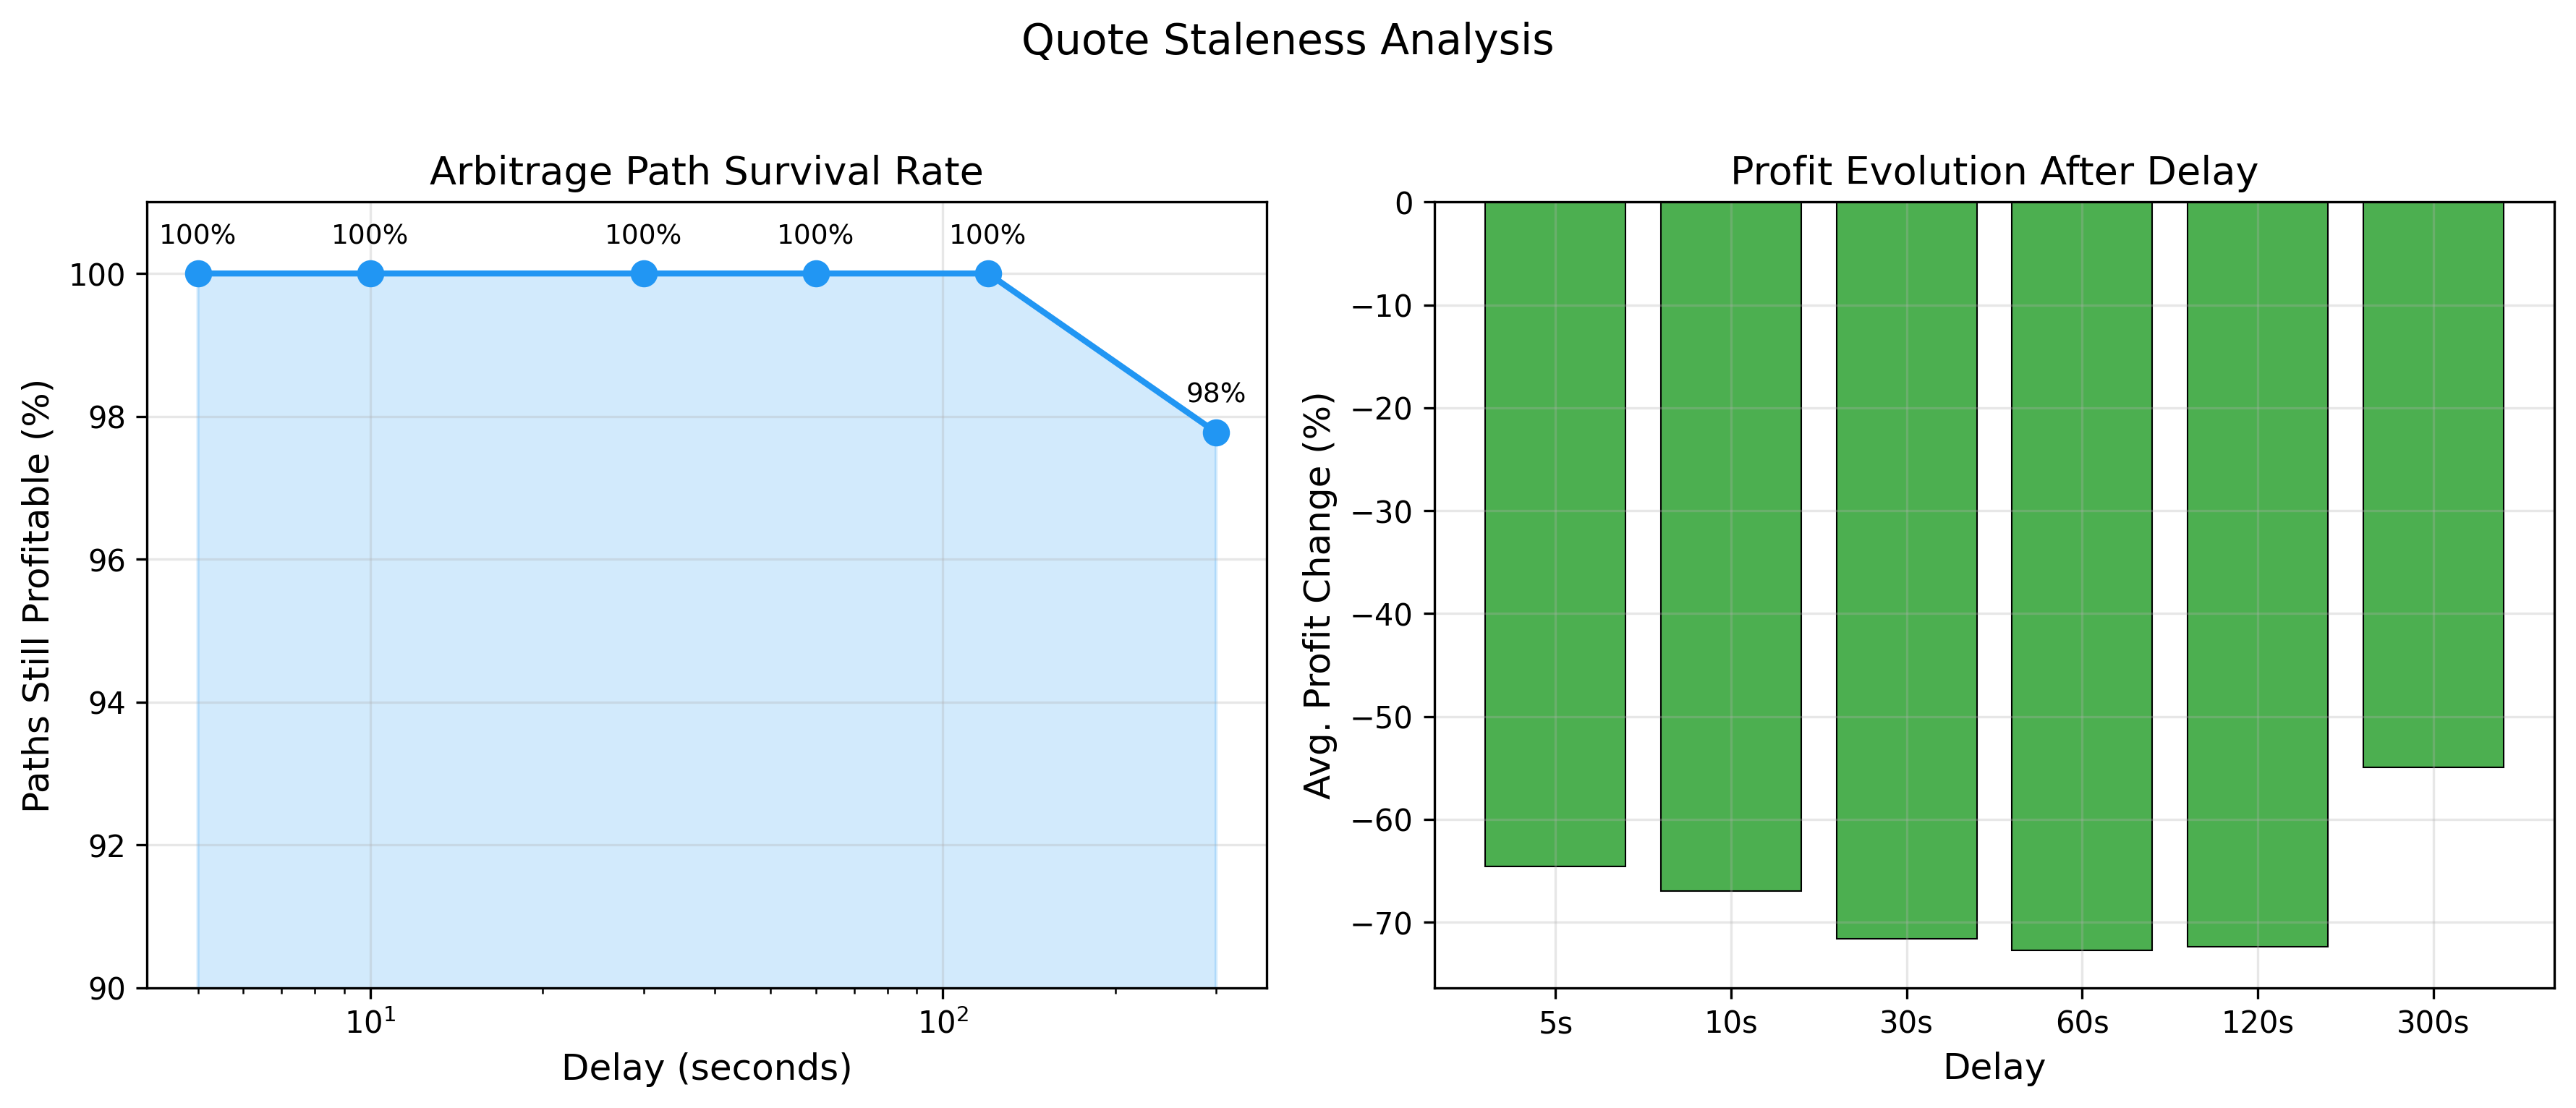
\includegraphics[width=\linewidth]{figures/fig09_quote_staleness.png}
    \caption{Quote staleness analysis: profit change and survival rate as a function of re-evaluation delay (5--300\,s). Paths remain profitable at all tested latencies.}
    \label{fig:staleness}
\end{figure}

\subsubsection{Temporal Robustness: 8-Hour Overnight Test}
\label{sec:overnight}

To move beyond single-snapshot evaluation, we execute an 8-hour continuous data collection campaign (96~snapshots at 5-minute intervals) running all five methods—$h_1$, $h_2$, $h_4$, Dijkstra, and 3-hop enumeration—from 5~preferred start nodes at three cash levels (\$1{,}000, \$10{,}000, \$100{,}000). This yields \textbf{7{,}200 search instances} (1{,}440 per method), providing distributional evidence of performance across changing market conditions.

\paragraph{Success rates.}
All four A*-based methods achieve a \textbf{100\% success rate} across all 1{,}440 runs per heuristic. The 3-hop enumeration baseline succeeds in only 573/1{,}440 runs (\textbf{39.8\%}), failing entirely for 3~of~5 start nodes because its fixed path template cannot discover 2-hop intra-exchange opportunities or 4+~hop routes.

\paragraph{Cross-exchange vs.\ intra-exchange paths.}
An important distinction emerges when we classify successful paths by type (Table~\ref{tab:overnight_pathtype}). Of 6{,}333 successful runs, 20.7\% discover \emph{intra-exchange} paths (single-hop trades like \texttt{kucoin:USDT}$\to$\texttt{kucoin:TUSD}) that exploit minor stablecoin depegging within a single exchange. These do not require cross-exchange transfers and are discoverable by trivial price comparisons. The remaining 79.3\% are genuine \emph{cross-exchange} paths involving transfers between exchanges.

\begin{table}[t]
\centering
\small
\caption{Overnight path-type breakdown by heuristic (1{,}440~runs each). Cross-exchange paths have $\geq$3~nodes; intra-exchange paths have 2~nodes.}
\label{tab:overnight_pathtype}
\begin{tabular}{lrrr}
\toprule
\textbf{Method} & \textbf{Cross-Exch.} & \textbf{Intra-Exch.} & \textbf{Cross \%} \\
\midrule
$h_2$ (slippage) &  1{,}378 &   62 & 95.7\% \\
Dijkstra         &  1{,}254 &  186 & 87.1\% \\
$h_1$ (liquidity)&    966 &  474 & 67.1\% \\
$h_4$ (Weighted) &    849 &  591 & 58.9\% \\
3-hop enum.      &    573 &    0 & 100\% \\
\bottomrule
\end{tabular}
\end{table}

$h_2$ produces the highest fraction of cross-exchange paths (95.7\%), suggesting that order-book-informed guidance effectively steers search toward multi-exchange opportunities. $h_4$ and $h_1$ more frequently settle on intra-exchange trades, as their penalty terms can make cross-exchange transfer edges look prohibitively costly.

\paragraph{Profit comparison (cross-exchange only).}
Restricting to cross-exchange paths: Dijkstra discovers the highest mean profit (\$42.42), followed by $h_2$ (\$39.15), $h_1$ (\$34.97), $h_4$ (\$22.16), and 3-hop (\$20.76). The lower profit for $h_1$ and $h_4$ reflects their penalty-driven exploration of safer but less profitable routes.

\paragraph{Latency profile — the key differentiator.}
The most striking result from the overnight campaign is the \emph{wall-clock latency} of each method under live market conditions, where heuristic API calls are not cached. Table~\ref{tab:latency} reports the full latency distribution.

\begin{table}[t]
\centering
\small
\caption{Wall-clock search latency over 1{,}440 live overnight runs per method. $h_1$ and $h_2$ exhibit extreme tail latency from order-book / volume API calls. $h_4$'s pre-computed scores produce Dijkstra-class latency with risk-aware guidance.}
\label{tab:latency}
\begin{tabular}{lrrrr}
\toprule
\textbf{Method} & \textbf{Median (s)} & \textbf{Mean (s)} & \textbf{P99 (s)} & \textbf{Max (s)} \\
\midrule
3-hop enum. & 0.001 & 0.001 & 0.001 & 0.009 \\
Dijkstra     & 0.012 & 0.013 & 0.017 & 0.212 \\
$h_4$        & 0.013 & 0.012 & 0.033 & 0.040 \\
$h_1$        & 0.022 & 0.446 & 6.900 & 8.590 \\
$h_2$        & 0.012 & 0.427 & 6.784 & 8.831 \\
\bottomrule
\end{tabular}
\end{table}

$h_4$ achieves a P99 latency of 33\,ms — comparable to Dijkstra (17\,ms) — because its chain transfer times and exchange reliability scores are pre-computed and cached via \texttt{lru\_cache}. By contrast, $h_1$ and $h_2$ suffer P99 latencies of \textbf{6.9--6.8\,s} (200$\times$ worse) due to live API calls that trigger on cache misses. In a live trading system where execution windows are measured in seconds, this latency profile makes $h_4$ the only viable heuristic-guided method for real-time deployment.

\paragraph{Search efficiency.}
$h_2$ achieves the fewest mean node expansions (269), outperforming Dijkstra (422) by 36\%. $h_4$ (413~expansions) and $h_1$ (617) expand more nodes due to their broader penalty structures. The 3-hop baseline averages 454~expansions per successful run.

\begin{figure}[t]
    \centering
    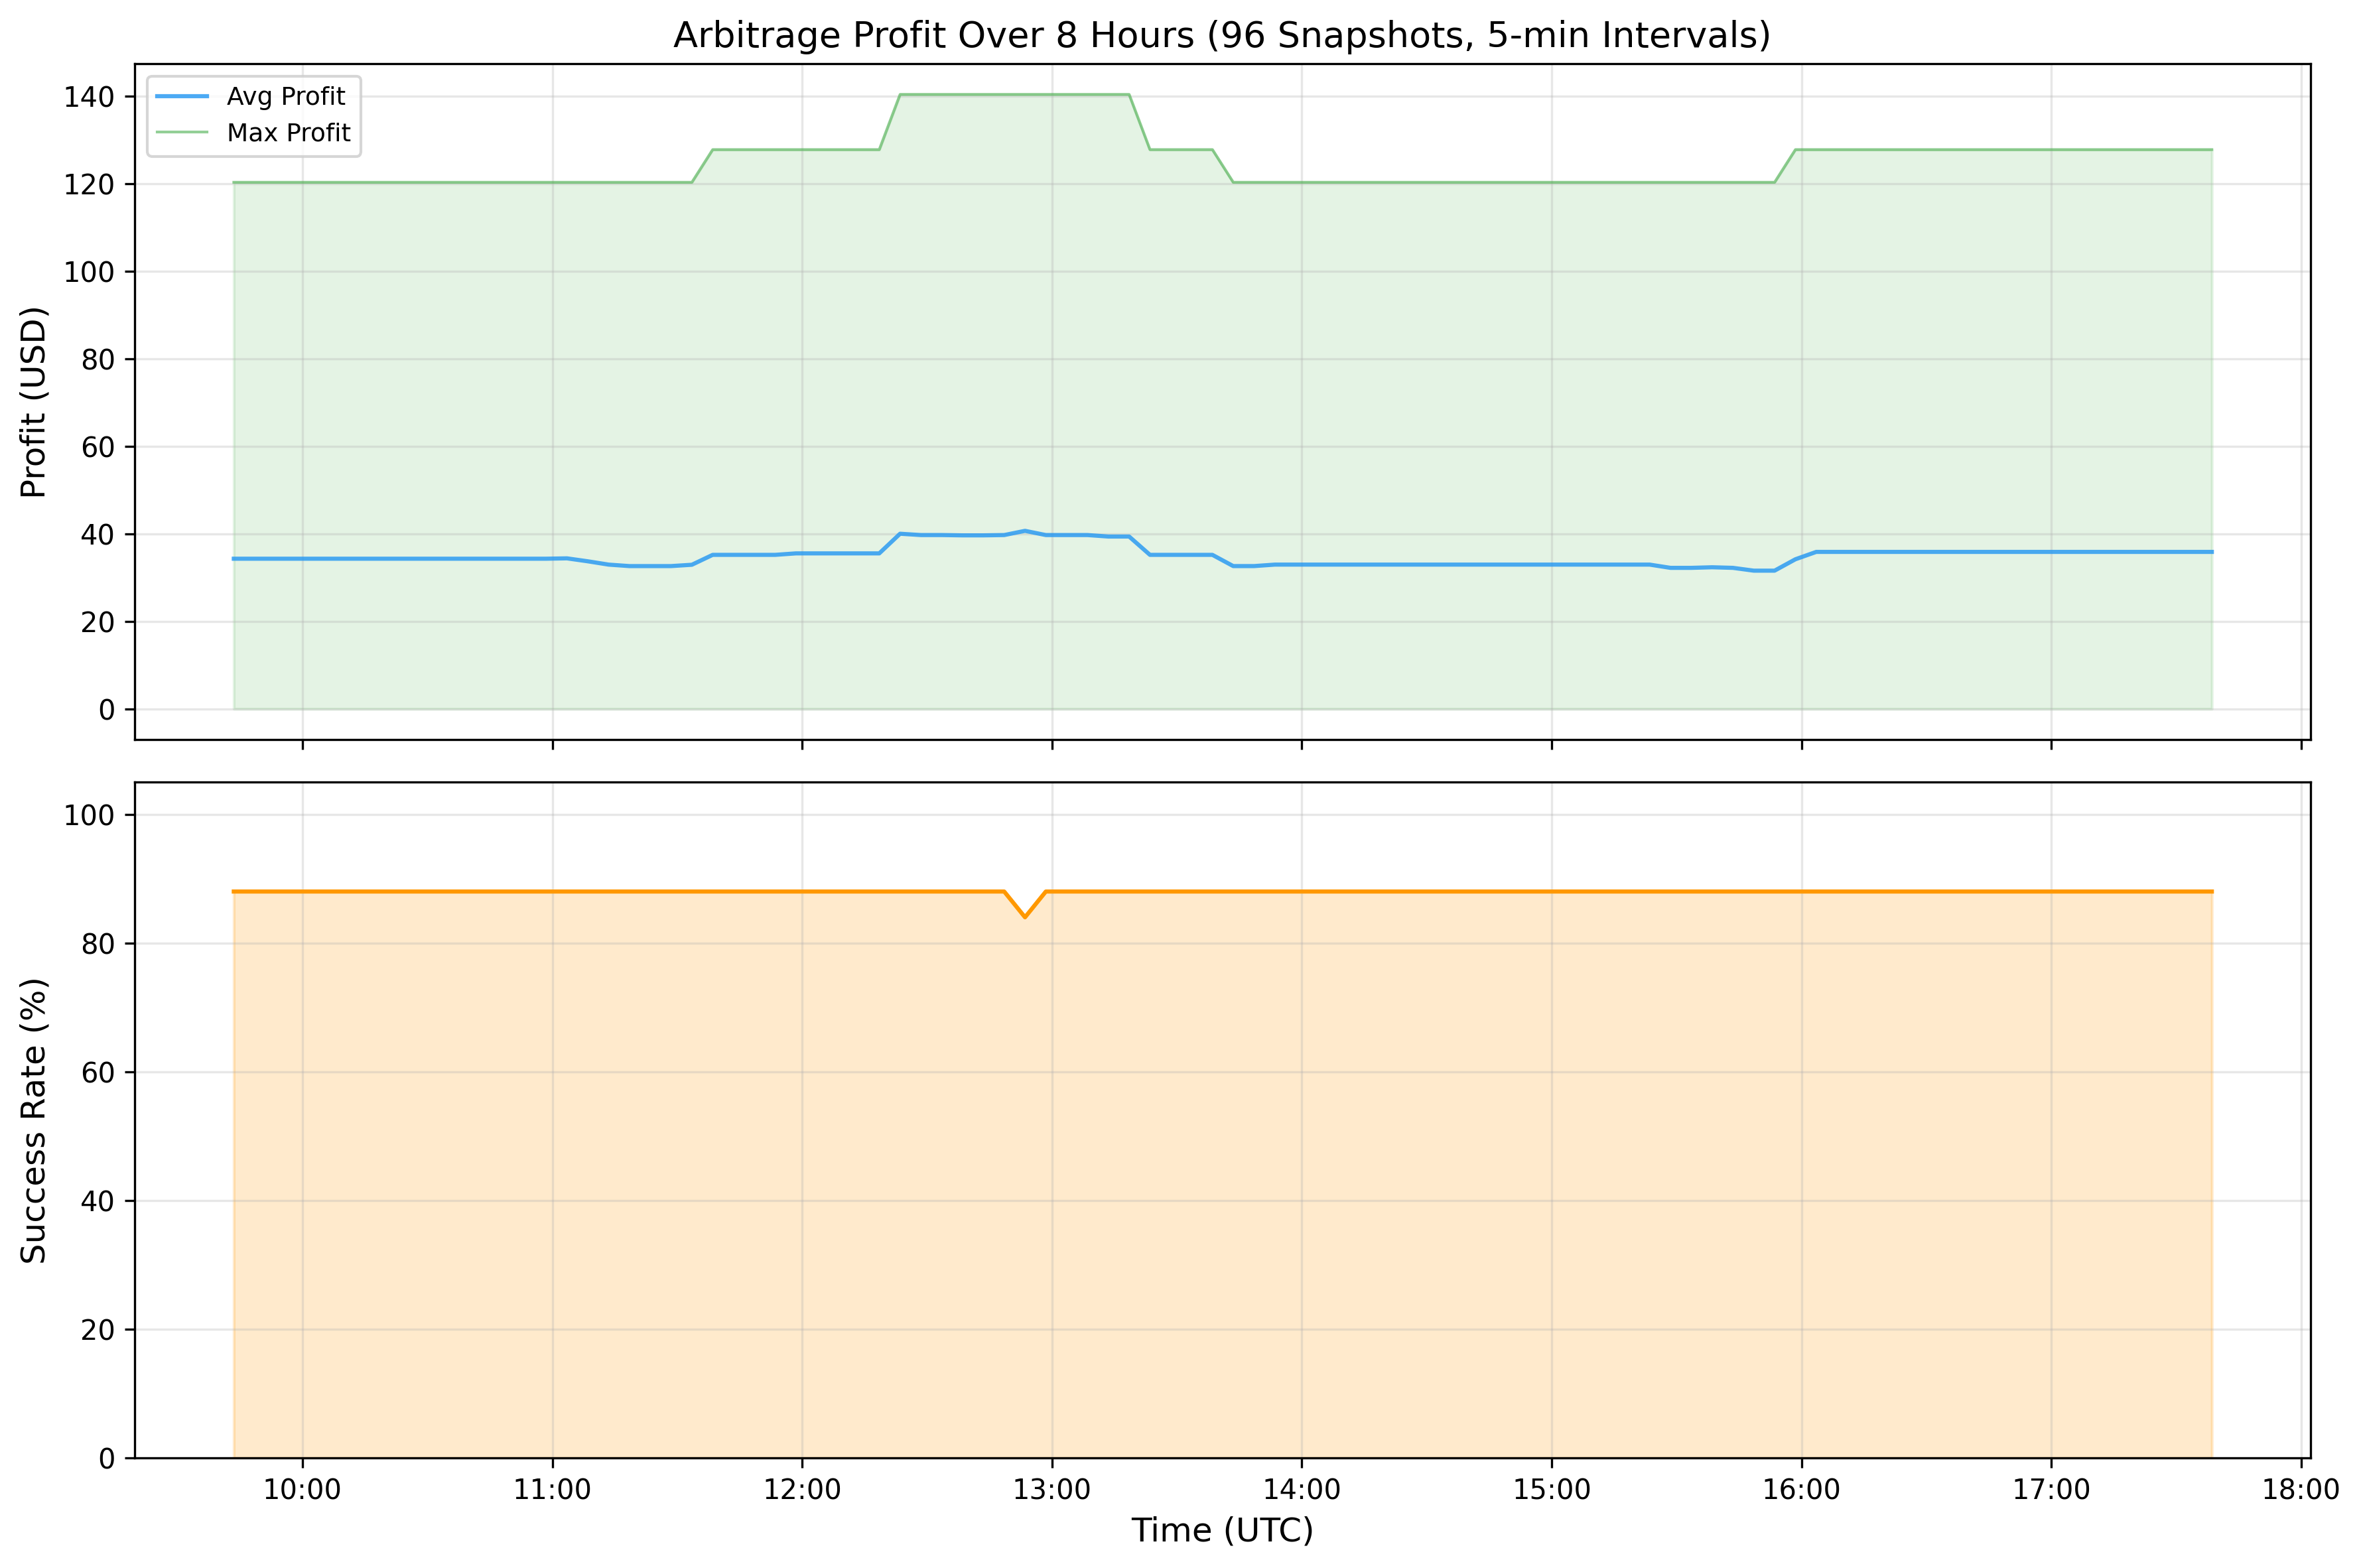
\includegraphics[width=\linewidth]{figures/fig10_overnight_timeseries.png}
    \caption{Profit time series over 8~hours (96~snapshots). Shaded bands show inter-quartile range across cash levels and start nodes. Opportunities persist throughout the observation window.}
    \label{fig:overnight_ts}
\end{figure}

\begin{figure}[t]
    \centering
    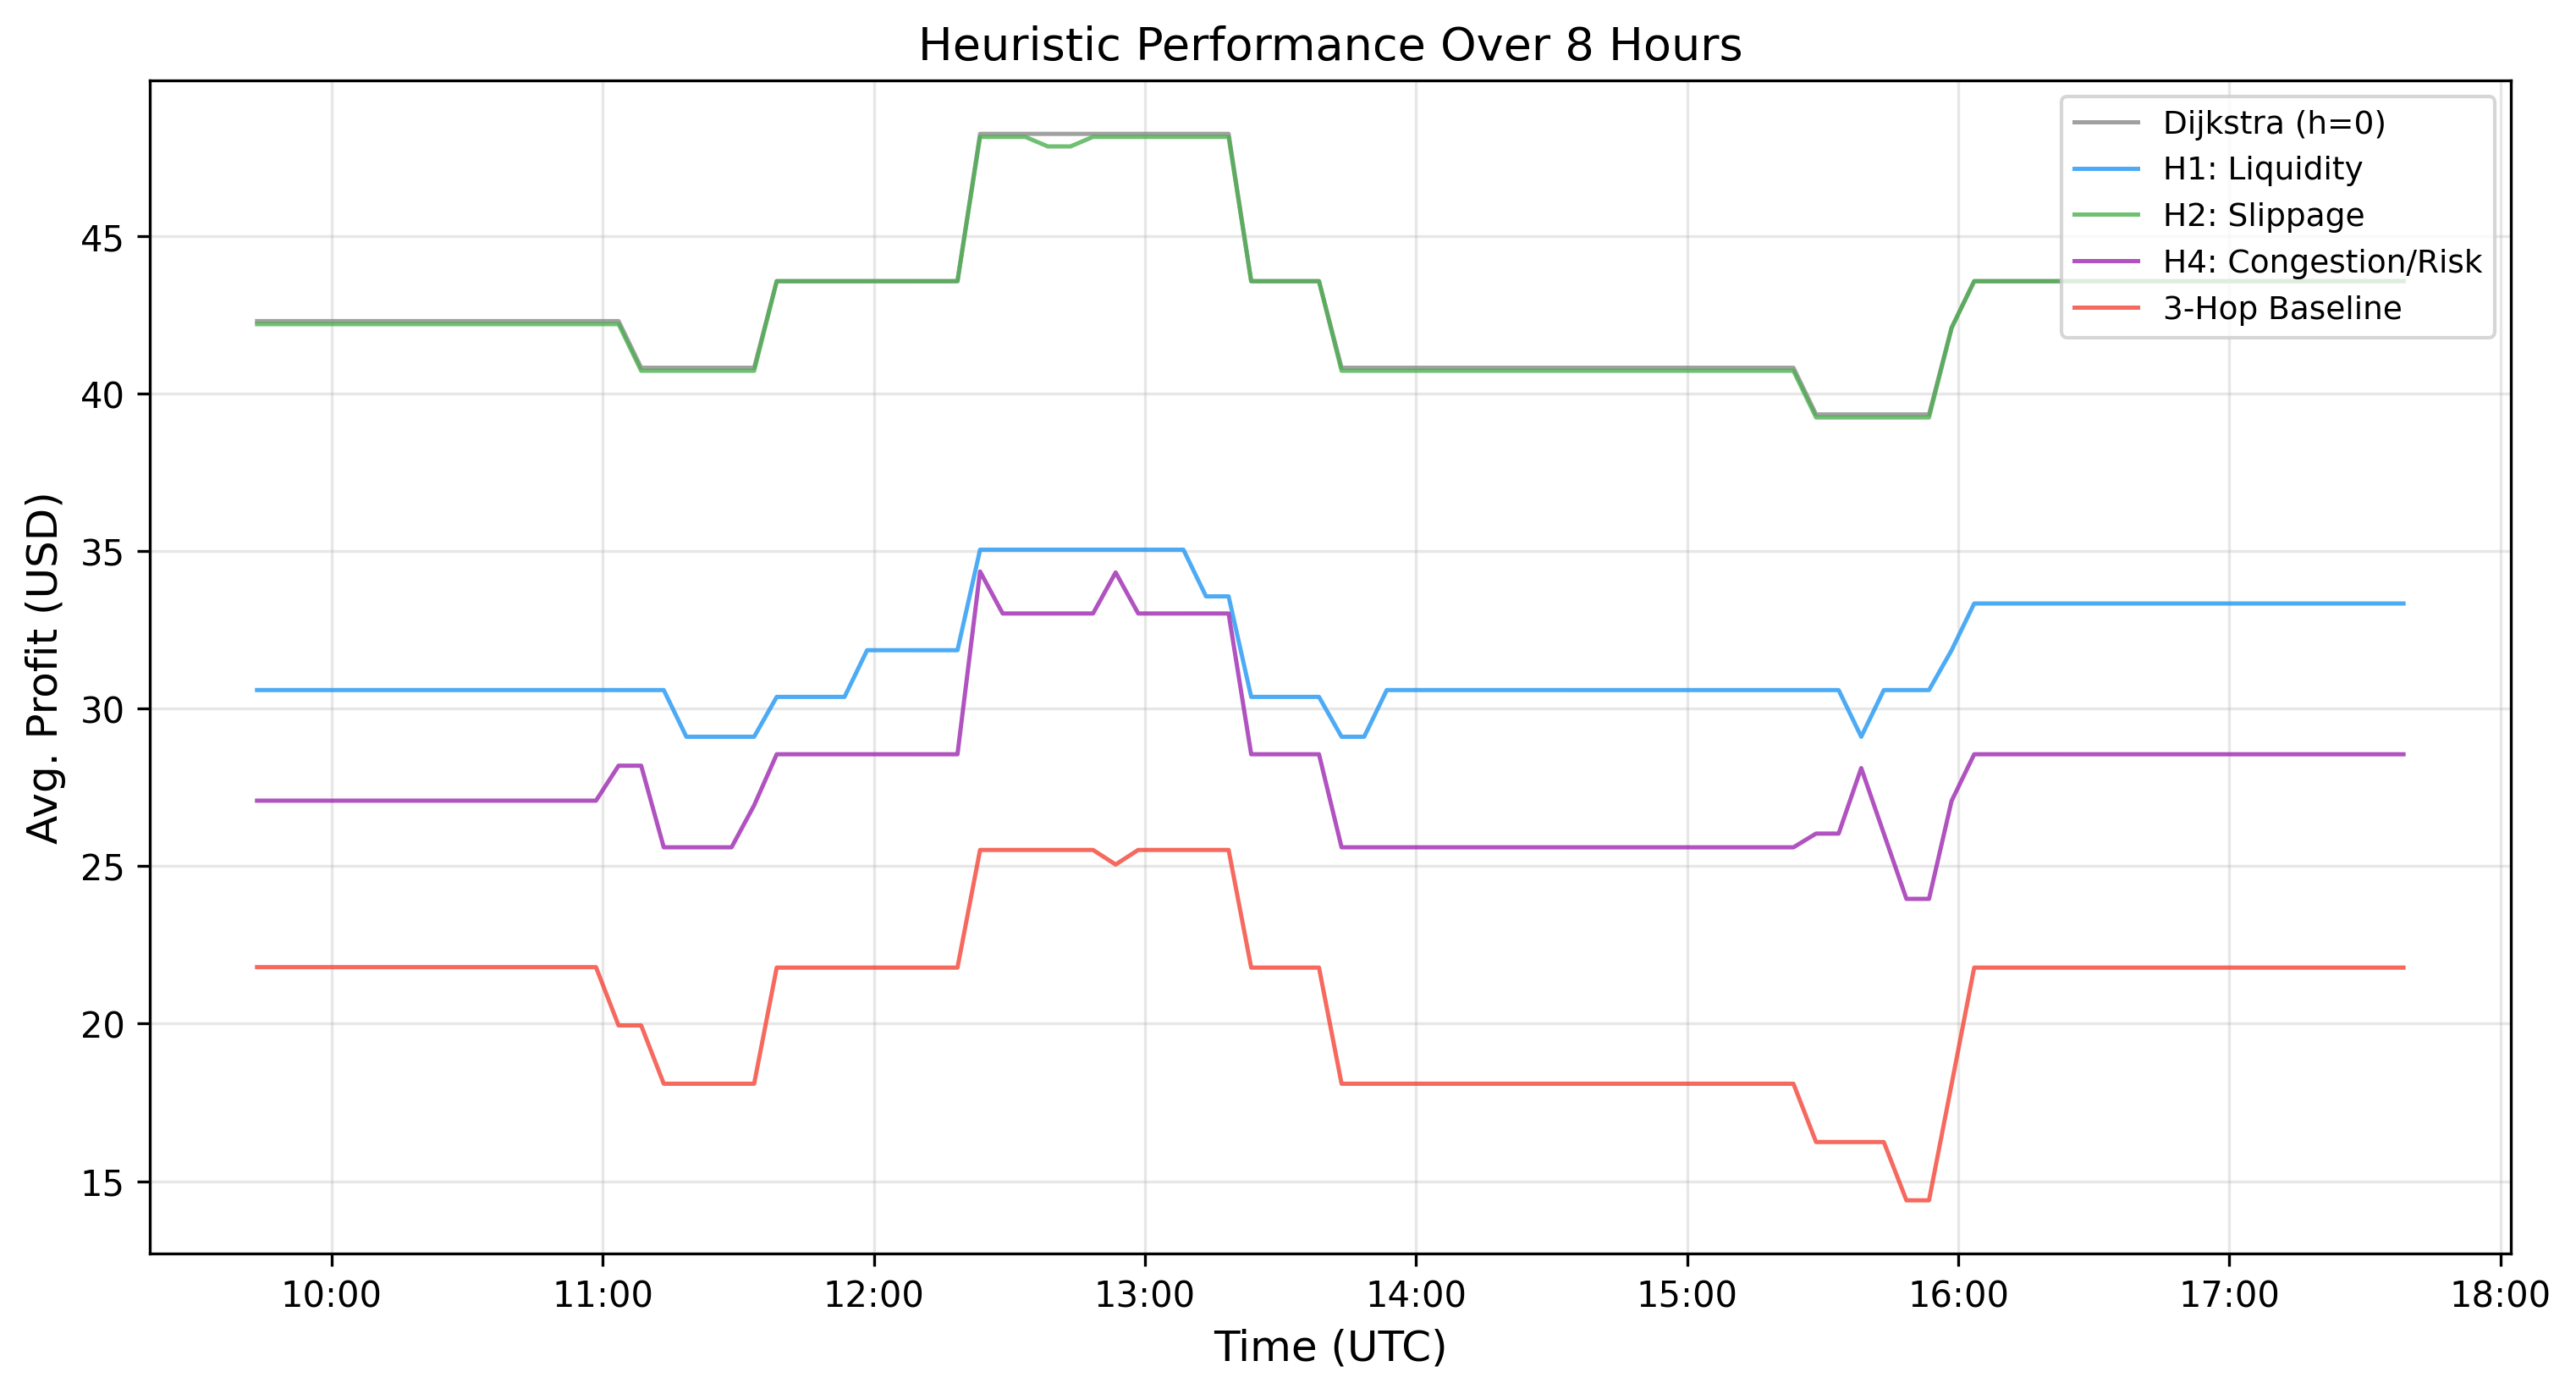
\includegraphics[width=\linewidth]{figures/fig11_overnight_heuristic_comparison.png}
    \caption{Overnight heuristic comparison: mean profit, success rate, and node expansions across 1{,}440 runs per method. $h_2$ provides the best profit-per-expansion ratio.}
    \label{fig:overnight_comparison}
\end{figure}

A key takeaway from the overnight campaign is that arbitrage opportunities are \emph{persistent}, not fleeting: profitable paths exist in every single 5-minute snapshot over the 8-hour window, though profit values cluster around a small number of structural optima (2--3 distinct profit levels per start node), reflecting the fee-dominated nature of stablecoin arbitrage.

\subsubsection{Sensitivity Analysis}
\label{sec:sensitivity}

We conduct four parameter sweeps on the 12-exchange graph to assess the robustness of our methods to hyperparameter choices, order size, and path depth constraints.

\paragraph{$h_1$ liquidity penalty weight $\lambda_{\text{liq}}$.}
Sweeping $\lambda_{\text{liq}} \in \{0.1, 0.5, 1.0, 2.0, 5.0\}$ across 25~trials per value, we find that profit and success rate are \emph{invariant} to the penalty weight: all five settings yield identical 80\% success rates and mean profit of \$27.77 (Figure~\ref{fig:sens_h1}). Node expansions increase modestly from 356 ($\lambda = 0.1$) to 376 ($\lambda = 5.0$), a difference of only 5.6\%. This stability arises because, in our graph, the liquidity penalty primarily reorders the open list without changing which paths are eventually explored.

\begin{figure}[t]
    \centering
    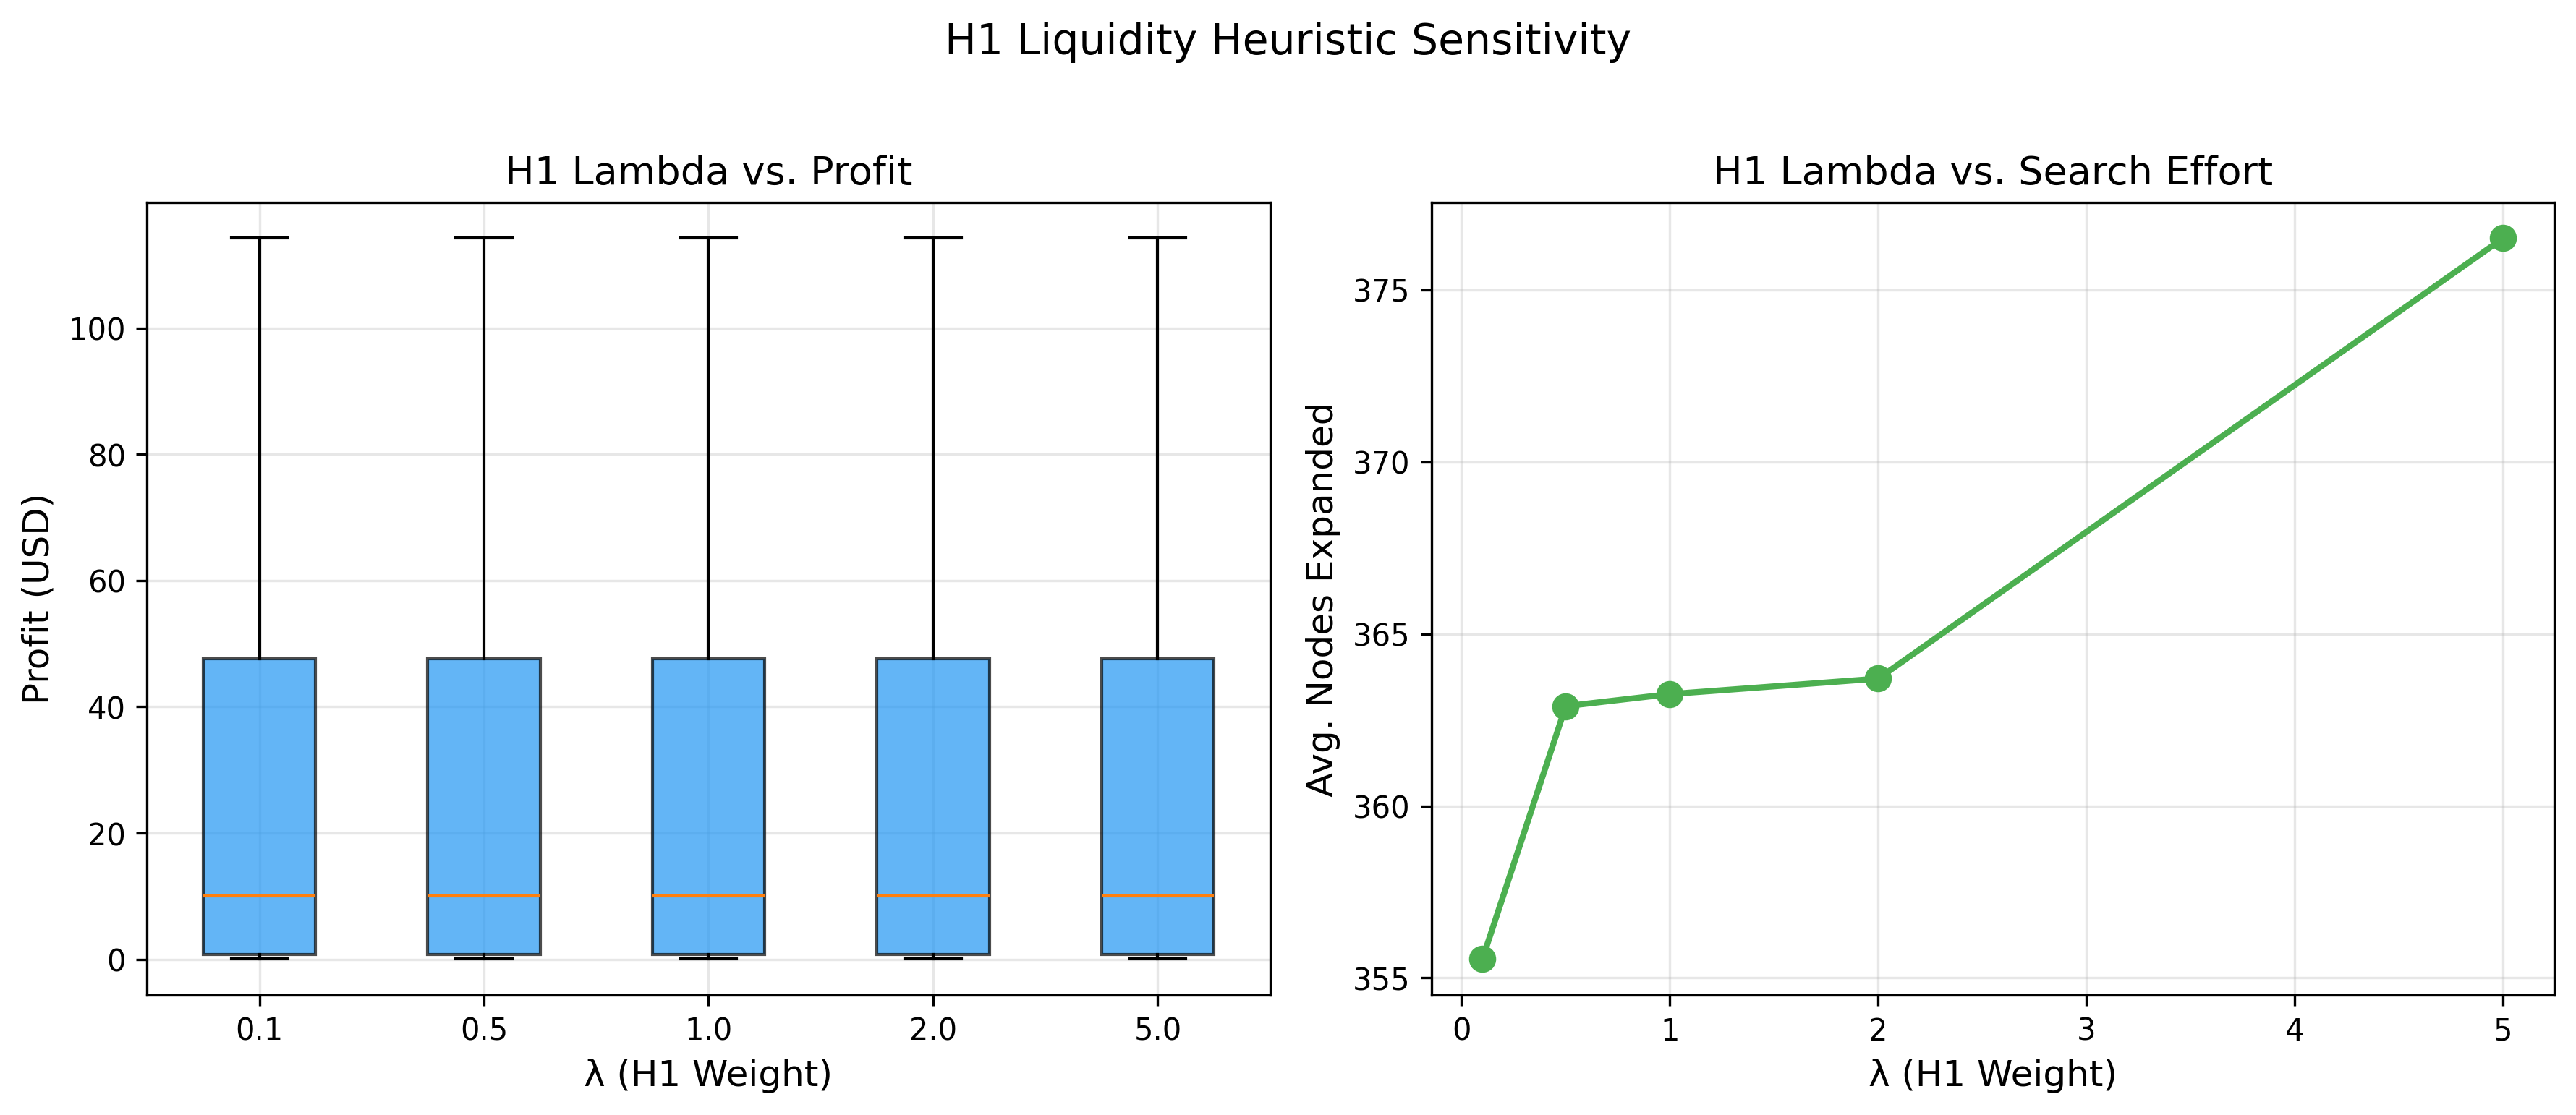
\includegraphics[width=\linewidth]{figures/fig12_sensitivity_h1_lambda.png}
    \caption{Sensitivity of $h_1$ to liquidity penalty weight $\lambda_{\text{liq}}$. Profit and success rate are invariant across a 50$\times$ range of $\lambda$ values.}
    \label{fig:sens_h1}
\end{figure}

\paragraph{$h_2$ slippage parameters ($\lambda_{\text{slip}}, \theta$).}
We jointly sweep the slippage penalty weight and tolerance threshold across a grid of values (100~configurations, Figure~\ref{fig:sens_h2}). Of these, 80\% produce successful paths. The heatmap reveals that moderate penalty weights ($\lambda_{\text{slip}} \in [0.3, 1.0]$) combined with moderate thresholds ($\theta \in [5, 20]$\,bps) form a broad plateau of high performance, indicating that $h_2$ is not sensitive to precise tuning.

\begin{figure}[t]
    \centering
    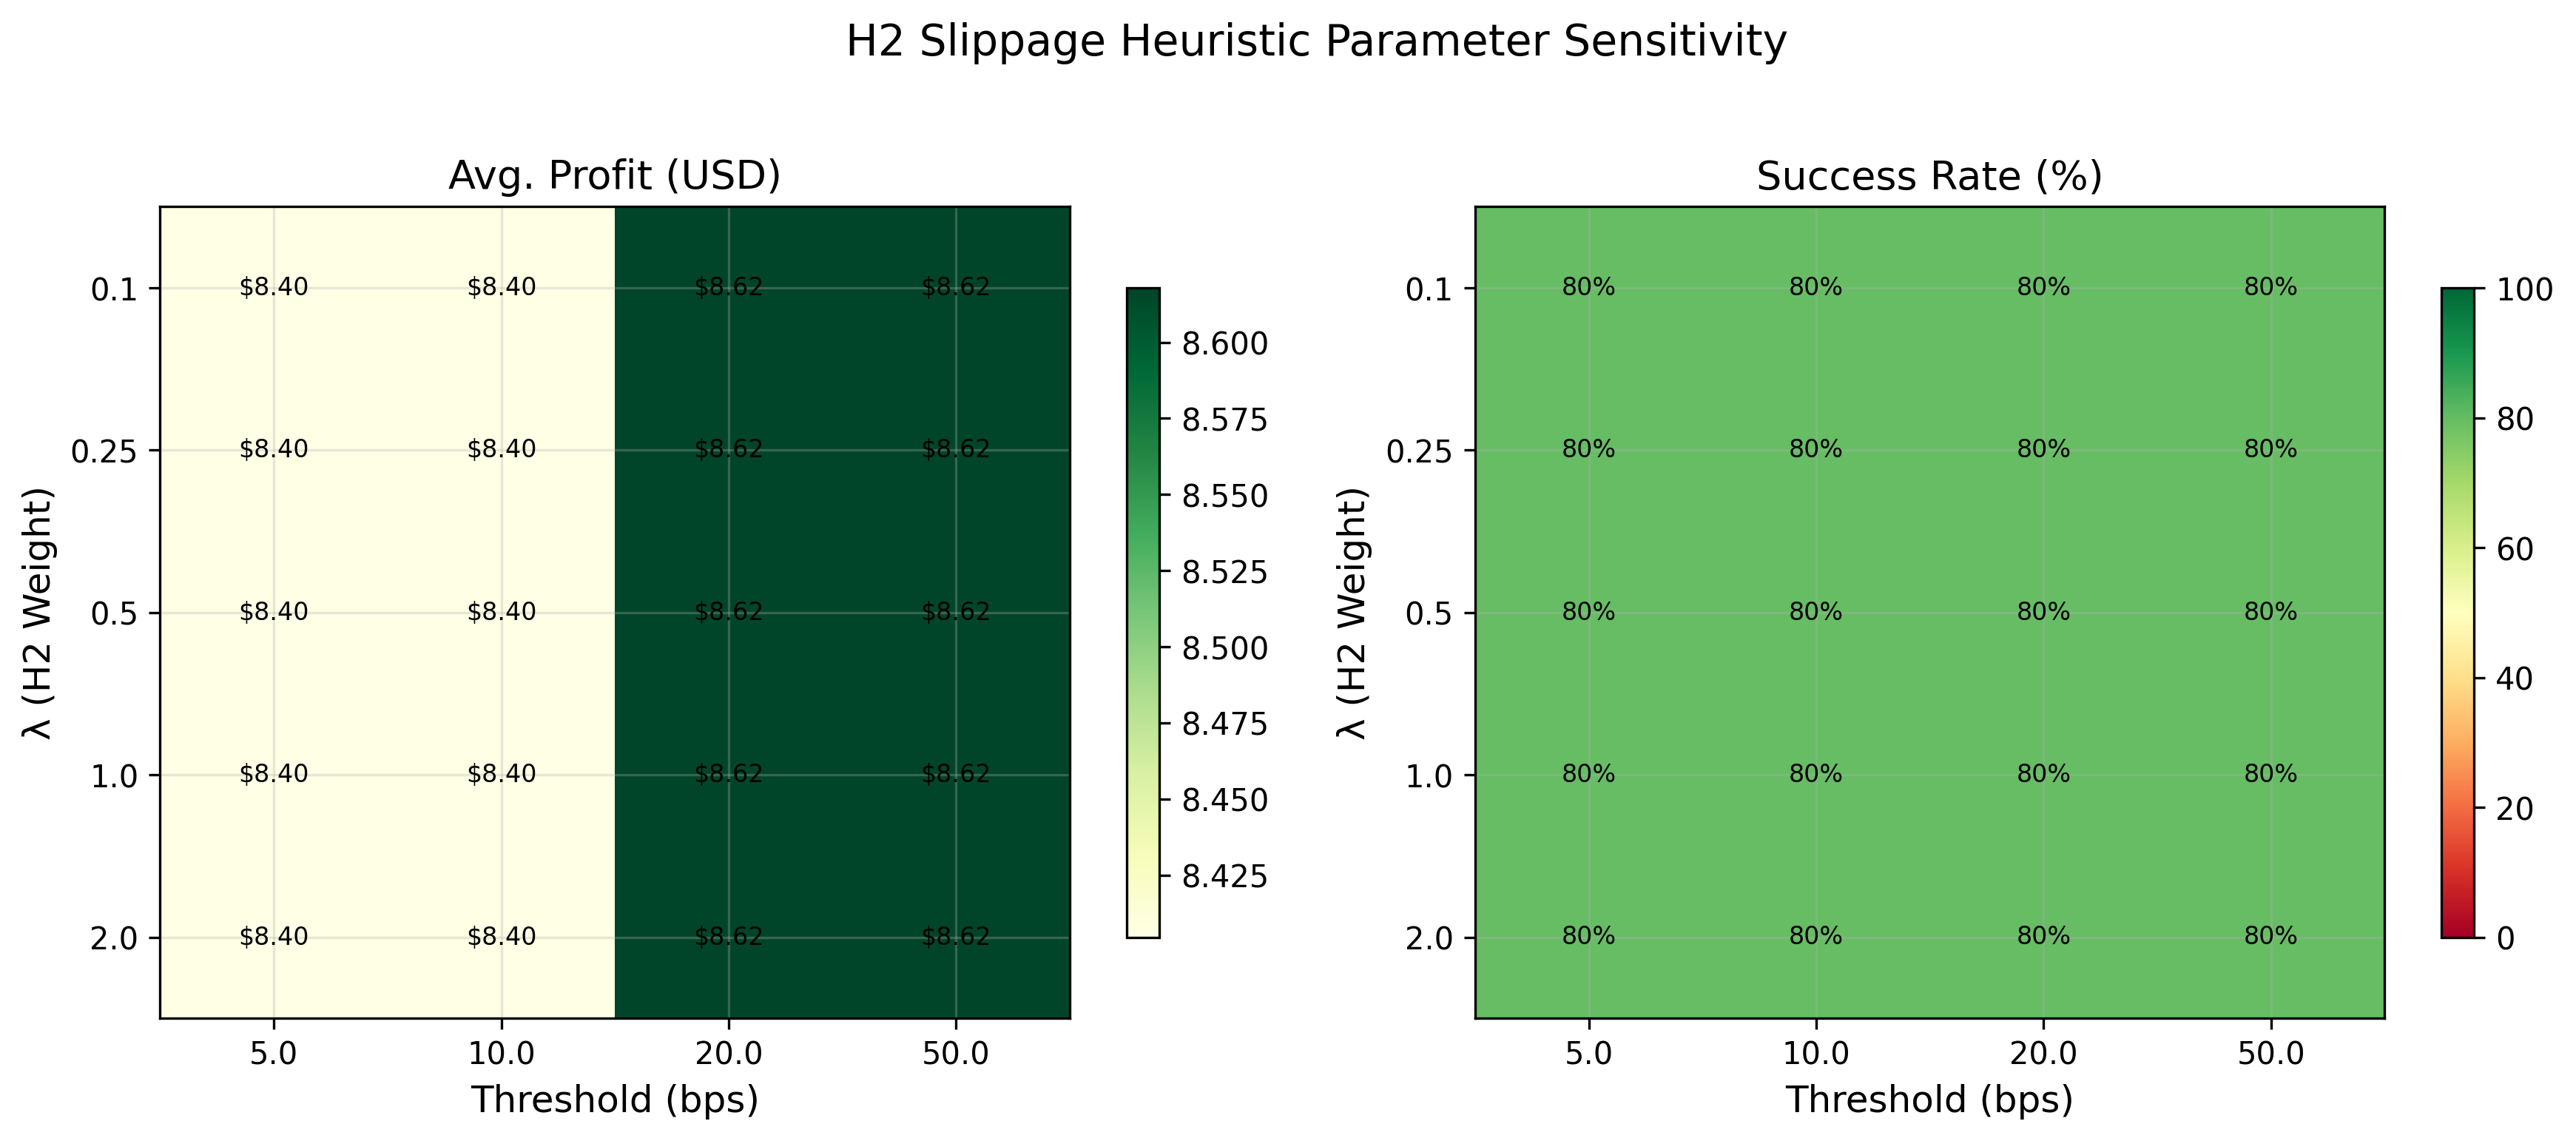
\includegraphics[width=\linewidth]{figures/fig13_sensitivity_h2_heatmap.png}
    \caption{$h_2$ sensitivity heatmap: success rate across $(\lambda_{\text{slip}}, \theta)$ parameter grid. A broad plateau of high success exists around moderate parameter values.}
    \label{fig:sens_h2}
\end{figure}

\paragraph{Order size.}
Sweeping order sizes from \$100 to \$100{,}000 across five levels, we observe that profit scales linearly with order size: \$0.09 at \$100, \$0.86 at \$1{,}000, \$8.62 at \$10{,}000, \$43.09 at \$50{,}000, and \$86.18 at \$100{,}000 (Figure~\ref{fig:sens_order}). The success rate remains constant at 80\% (4/5 start nodes), confirming that path selection is independent of order size within the tested range—slippage costs at these volumes do not materially alter the optimal path structure.

\begin{figure}[t]
    \centering
    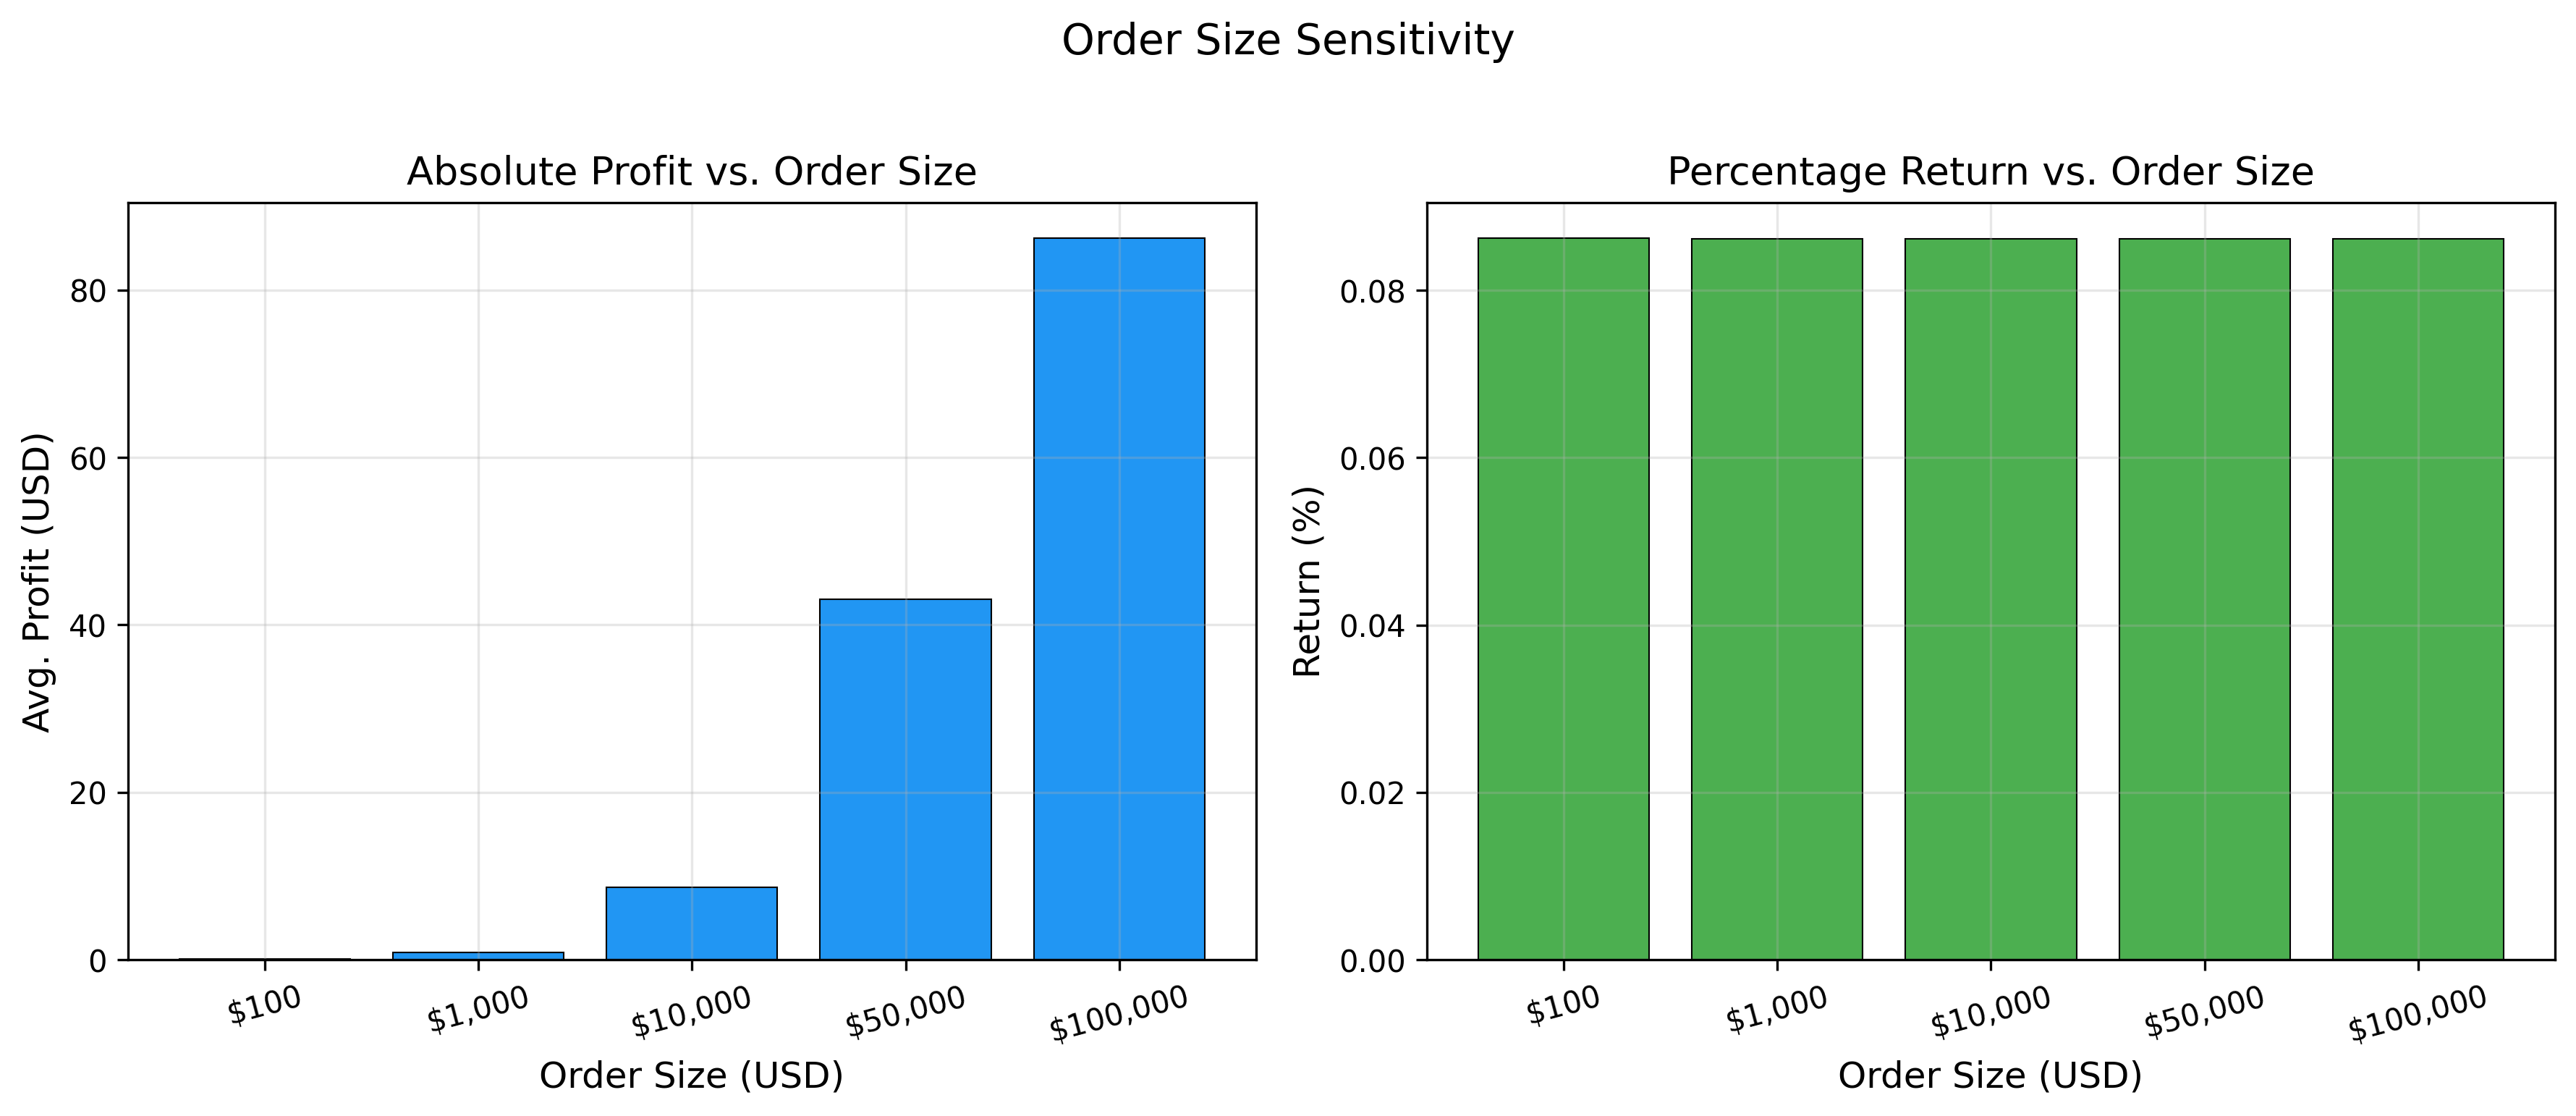
\includegraphics[width=\linewidth]{figures/fig14_sensitivity_order_size.png}
    \caption{Mean profit as a function of order size (\$100--\$100k). Profit scales linearly, and success rate is constant at 80\%.}
    \label{fig:sens_order}
\end{figure}

\paragraph{Maximum path depth.}
Varying the depth limit from 3 to 6 hops, we find that 4/5 start nodes produce profitable paths at \emph{all} depths, with identical optimal paths across configurations (Figure~\ref{fig:sens_depth}). This confirms the earlier observation that profitable stablecoin arbitrage paths are inherently short (3~hops), and increasing the depth limit does not improve outcomes—it merely expands the search space without yielding longer profitable structures.

\begin{figure}[t]
    \centering
    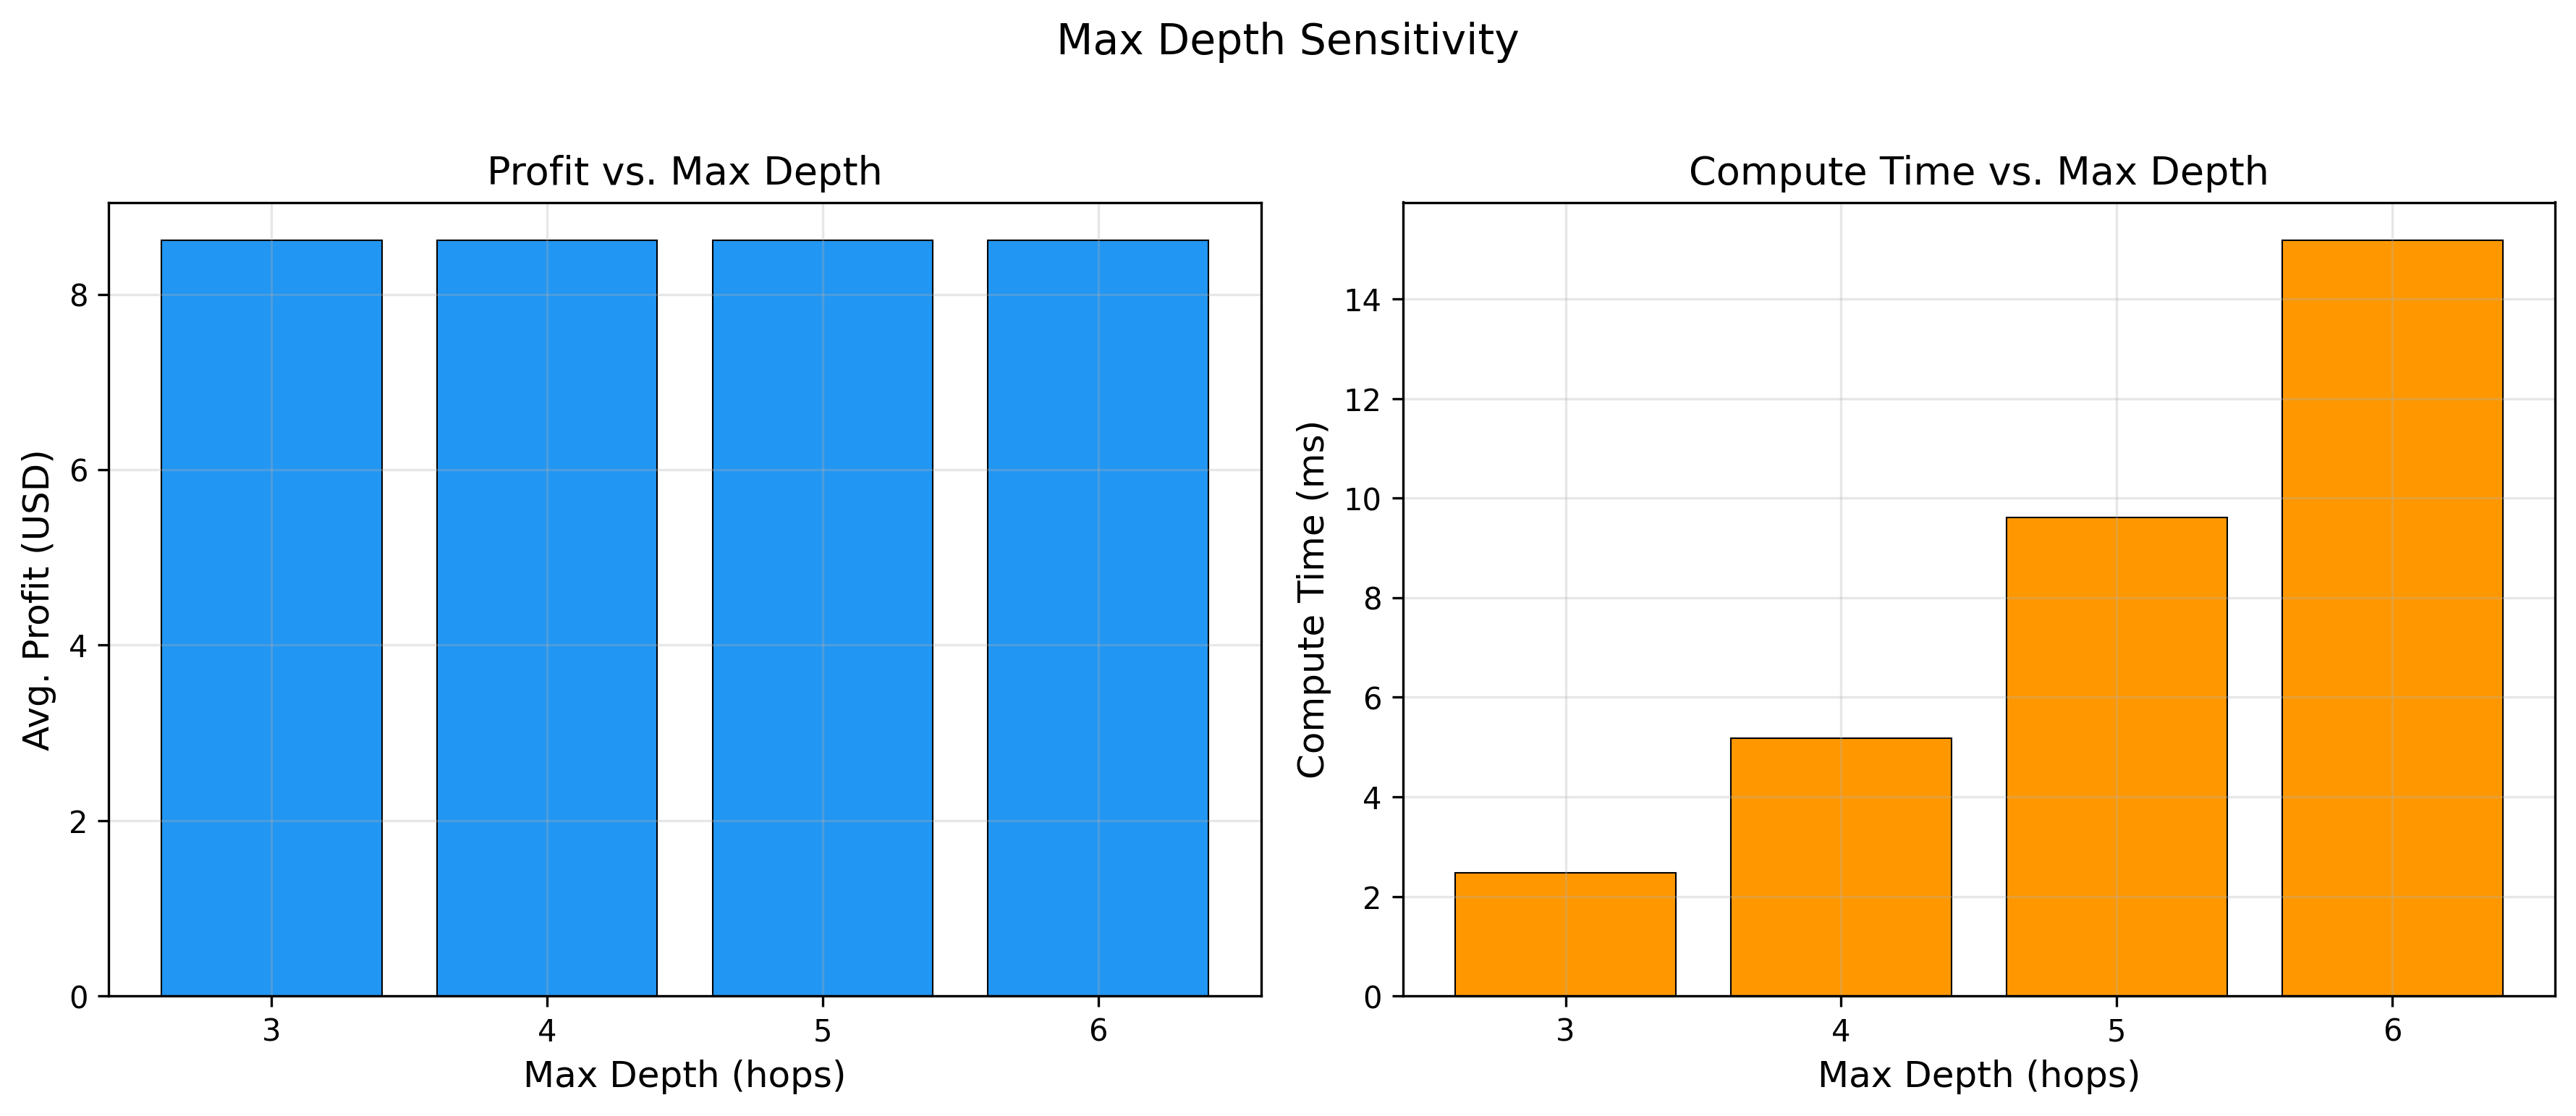
\includegraphics[width=\linewidth]{figures/fig15_sensitivity_max_depth.png}
    \caption{Effect of maximum path depth on success rate and profit. Performance is stable across depths 3--6, confirming that optimal paths are consistently 3 hops.}
    \label{fig:sens_depth}
\end{figure}

